\chapter{Cellules souches, régénération et vieillissement}\label{ch:b3:stem-cells}

Coupez la patte d'un axolotl et en deux mois il en a fait pousser une
neuve, os, muscle, nerf et peau aux bons endroits, et il recommencera
aussi souvent que vous couperez. Coupez une planaire en vingt morceaux
et chacun devient un ver entier en quinze jours, le morceau qui était
une queue faisant repousser une tête avec des yeux et un cerveau.
Coupez un doigt humain au-dessus de la dernière articulation et il
cicatrise. Pourtant le corps humain n'est pas sans renouvellement~:
chaque seconde il fabrique deux millions de globules rouges, la muqueuse
de l'intestin est remplacée tous les cinq jours, la peau tous les mois,
et tout cela descend de petites populations de cellules qui se divisent
la vie durant sans s'épuiser. Ce chapitre traite de ces cellules --- ce
qui fait une \omterm{def:b3:stem-cells:stem}{cellule souche}, comment sa \omterm{def:b3:stem-cells:stem}{niche} la garde, comment toute la
hiérarchie du sang ou de l'intestin se bâtit à partir d'elle ---, des
animaux qui savent refaire pousser ce que nous ne savons pas et pourquoi,
de la découverte que n'importe quelle cellule peut être ramenée à l'état
embryonnaire par quatre gènes, et de ce que l'arithmétique de la division
cellulaire a à dire sur les raisons de notre vieillissement.

\section{Ce qu'est une cellule souche}

\begin{definition}[Les cellules souches et leur hiérarchie]\label{def:b3:stem-cells:stem}
\index{cellule souche}\index{auto-renouvellement}\index{division asymétrique}\index{progéniteur}\index{cellule d'amplification transitoire}\index{niche}
Une \emph{cellule souche} a deux propriétés qui la définissent~: elle
peut s'\emph{auto-renouveler}, en produisant des filles qui sont des
cellules souches, et elle peut produire des filles qui se différencient.
Elle peut faire les deux à la fois, par \emph{division asymétrique}, une
fille de chaque sorte, le destin étant décidé par l'héritage inégal de
déterminants ou par la fille qui reste au contact de la \emph{niche} ---
le microenvironnement de cellules voisines, de matrice et de signaux qui
maintient une cellule à l'état souche~; ou bien elle peut se diviser
symétriquement, certaines divisions donnant deux cellules souches et
d'autres deux cellules en différenciation, la population restant en
moyenne constante. Les filles qui se différencient passent d'ordinaire
par des stades de \emph{progéniteur} ou d'\emph{amplification
transitoire}, en se divisant encore plusieurs fois avec une potence qui
se rétrécit avant de mûrir~: la hiérarchie amplifie quelques divisions
lentes de cellules souches en une production abondante, et limite le
nombre de divisions que doit faire chaque cellule souche. Les cellules
souches adultes sont rares et lentes --- une cellule souche
hématopoïétique se divise peut-être une fois par an, une cellule souche
intestinale une fois par jour --- et \emph{multipotentes}, confinées aux
lignées de leur tissu~; les \omterm{def:b3:stem-cells:pluripotency}{cellules souches embryonnaires}, issues de la
masse cellulaire interne du blastocyste, sont \emph{pluripotentes},
capables de faire tous les tissus du corps mais non le placenta.
\end{definition}

\begin{omfigure}
\begin{tikzpicture}[every node/.style={font=\scriptsize}, >=stealth]
  \node[draw, very thick, rounded corners, fill=omDef!25, align=center] (hsc) at (0,3.6) {cellule souche hématopoïétique\\$\sim$\num{10000} chez l'humain~; se divise $\sim$ une fois par an};
  \node[draw, thick, rounded corners, fill=omDef!12, align=center] (mpp) at (0,2.4) {progéniteurs multipotents};
  \node[draw, thick, rounded corners, fill=omThm!15, align=center] (cmp) at (-3.2,1.2) {progéniteur myéloïde};
  \node[draw, thick, rounded corners, fill=omProp!20, align=center] (clp) at (3.2,1.2) {progéniteur lymphoïde};
  \node[align=center, font=\tiny] (e) at (-5.4,-0.4) {érythrocytes\\$2\times 10^{11}$/jour};
  \node[align=center, font=\tiny] (pl) at (-3.6,-0.4) {plaquettes\\(mégacaryocytes)};
  \node[align=center, font=\tiny] (g) at (-1.8,-0.4) {granulocytes\\$10^{11}$/jour};
  \node[align=center, font=\tiny] (m) at (-0.2,-0.4) {monocytes,\\macrophages};
  \node[align=center, font=\tiny] (b) at (1.8,-0.4) {lymphocytes B};
  \node[align=center, font=\tiny] (t) at (3.4,-0.4) {lymphocytes T};
  \node[align=center, font=\tiny] (nk) at (5.0,-0.4) {cellules NK};
  \draw[->, thick] (hsc) -- (mpp); \draw[->, thick] (mpp) -- (cmp); \draw[->, thick] (mpp) -- (clp);
  \foreach \x in {e,pl,g,m} { \draw[->, thick] (cmp) -- (\x); }
  \foreach \x in {b,t,nk} { \draw[->, thick] (clp) -- (\x); }
  \draw[->, thick, omDef!70!black] (hsc.west) .. controls (-3.0,4.4) and (-3.0,3.0) .. (hsc.south west) node[pos=0.5, left, font=\tiny, omDef!70!black, align=right] {auto-renouvellement};
  \node[right, align=left, font=\tiny] at (4.4,3.6) {chaque étage se divise plus souvent\\et a une potence plus étroite~;\\$\sim 20$ divisions de la cellule souche\\au globule rouge, de sorte qu'une seule\\division souche donne $\sim 10^{6}$ cellules};
\end{tikzpicture}

{\small La hiérarchie hématopoïétique. Quelques milliers de \omterm{def:b3:stem-cells:stem}{cellules
souches} lentes de la moelle alimentent des \omterm{def:b3:stem-cells:stem}{progéniteurs} qui se divisent
vite et s'engagent progressivement, de sorte que la production de mille
milliards de cellules par jour ne coûte presque rien aux \omterm{def:b3:stem-cells:stem}{cellules
souches}.}
\end{omfigure}

\begin{proof}[Faits expérimentaux]
Till et McCulloch (1961) injectèrent des cellules de moelle à des souris
irradiées à dose létale et comptèrent dix jours plus tard les nodules
apparus sur la rate~: chacun était une colonie de cellules sanguines de
plusieurs lignées, leur nombre proportionnel aux cellules injectées, et
le marquage des chromosomes du donneur montra que chaque colonie était
un clone --- une seule cellule avait fait des globules rouges, des
granulocytes et des plaquettes, et certaines colonies contenaient des
cellules capables de semer de nouvelles colonies chez une seconde
souris~: \omterm{def:b3:stem-cells:stem}{auto-renouvellement} et multipotence dans une seule cellule, la
définition opératoire d'une \omterm{def:b3:stem-cells:stem}{cellule souche}, et le fondement de la greffe
de moelle osseuse. Barker et Clevers (2007) marquèrent d'une couleur
héritable les cellules exprimant le gène \emph{Lgr5} à la base des
cryptes intestinales et virent, au fil des semaines, la couleur grimper
la crypte et remplir des villosités entières~: les cellules marquées
étaient les \omterm{def:b3:stem-cells:stem}{cellules souches} de l'intestin, et l'une d'elles, cultivée
dans un gel avec les trois bons facteurs de croissance, devint un
intestin miniature, un \emph{\omterm{def:b3:stem-cells:pluripotency}{organoïde}}, avec ses propres cryptes et
villosités (Sato, 2009).
\end{proof}

\begin{proposition}[La niche et la crypte]\label{prop:b3:stem-cells:crypt}
\index{crypte}\index{Lgr5}\index{cellule de Paneth}\index{signalisation Wnt}\index{dérive neutre}
La \emph{crypte} intestinale est la \omterm{def:b3:stem-cells:stem}{niche} la mieux comprise. À sa base
une quinzaine de \omterm{def:b3:stem-cells:stem}{cellules souches} \emph{Lgr5} sont calées entre des
\omterm{prop:b3:stem-cells:crypt}{cellules de Paneth}, qui sécrètent les signaux Wnt et Notch et les
facteurs de croissance qui les gardent souches~; une \omterm{def:b3:stem-cells:stem}{cellule souche}
poussée hors du contact des \omterm{prop:b3:stem-cells:crypt}{cellules de Paneth} perd le signal en
quelques diamètres cellulaires et devient une \omterm{def:b3:stem-cells:stem}{cellule d'amplification
transitoire}, qui se divise quatre ou cinq fois dans la crypte puis se
différencie en cellules absorbantes et sécrétrices qui remontent la
villosité et sont larguées de sa pointe cinq jours plus tard. Les
\omterm{def:b3:stem-cells:stem}{cellules souches} se divisent symétriquement, environ une fois par jour,
et rivalisent pour une place limitée dans la \omterm{def:b3:stem-cells:stem}{niche}~: par hasard un clone
s'étend et les autres se perdent, si bien qu'en quelques mois chaque
crypte descend d'une seule \omterm{def:b3:stem-cells:stem}{cellule souche} --- une \emph{\omterm{prop:b3:stem-cells:crypt}{dérive neutre}} à
l'échelle d'une crypte, une marche au hasard à frontières absorbantes.
C'est la \omterm{def:b3:stem-cells:stem}{niche}, et non la cellule, qui tient le caractère souche~:
remettez une cellule différenciée au contact des signaux des \omterm{prop:b3:stem-cells:crypt}{cellules de
Paneth} après une lésion et elle peut revenir en arrière~; sortez la
\omterm{def:b3:stem-cells:stem}{cellule souche} et donnez-lui les signaux dans une boîte et elle fait un
\omterm{def:b3:stem-cells:pluripotency}{organoïde}. La moelle osseuse, les follicules pileux, le testicule et les
zones de \omterm{def:b3:stem-cells:stem}{cellules souches} neurales du cerveau suivent la même logique
avec d'autres signaux.
\end{proposition}
\begin{proof}[Faits expérimentaux]
Snippert et ses collègues (2010) marquèrent les \omterm{def:b3:stem-cells:stem}{cellules souches} des
cryptes d'un «~confetti~» de quatre couleurs au hasard~; les cryptes
étaient d'abord multicolores et étaient devenues monochromes en quelques
mois, à un rythme compatible avec une division symétrique et une
compétition neutre entre une quinzaine de cellules --- plutôt qu'avec
une \omterm{def:b3:stem-cells:stem}{division asymétrique}, qui aurait gardé indéfiniment chaque couleur.
Retirer les \omterm{prop:b3:stem-cells:crypt}{cellules de Paneth} rétrécit le réservoir de \omterm{def:b3:stem-cells:stem}{cellules
souches}~; retirer le signal Wnt vide la crypte en quelques jours.
\end{proof}

\begin{omfigure}
\begin{tikzpicture}[every node/.style={font=\scriptsize}, >=stealth]
  % crypt-villus
  \draw[very thick, omDef] (0,-2.6) .. controls (0,-0.4) and (0.4,0) .. (0.8,0) -- (0.8,3.6) .. controls (0.8,4.1) and (1.6,4.1) .. (1.6,3.6) -- (1.6,0) .. controls (2.0,0) and (2.4,-0.4) .. (2.4,-2.6);
  \draw[very thick, omDef] (0,-2.6) arc[start angle=180, end angle=360, radius=1.2];
  % stem cells at base
  \foreach \a in {200,230,260,290,320} { \fill[omThm!60] ({1.2+1.05*cos(\a)},{-2.6+1.05*sin(\a)}) circle (0.14); }
  \foreach \a in {215,245,275,305} { \fill[omMeth!60] ({1.2+0.75*cos(\a)},{-2.6+0.75*sin(\a)}) circle (0.13); }
  \node[right, align=left, font=\tiny] at (2.6,-3.4) {base~: $\sim 14$ cellules souches \emph{Lgr5} (en rouge)\\calées entre des cellules de Paneth (en vert),\\qui fournissent Wnt, Notch, EGF};
  % TA zone
  \foreach \y in {-1.8,-1.3,-0.8,-0.3} { \fill[omProp!50] (0.35,\y) circle (0.11); \fill[omProp!50] (2.05,\y) circle (0.11); }
  \node[right, align=left, font=\tiny] at (2.6,-1.1) {zone d'amplification transitoire~:\\4 à 5 divisions, une par jour,\\au-delà des signaux de Paneth};
  % villus cells
  \foreach \y in {0.4,1.0,1.6,2.2,2.8} { \fill[omDef!40] (0.95,\y) circle (0.1); \fill[omDef!40] (1.45,\y) circle (0.1); }
  \node[right, align=left, font=\tiny] at (2.6,1.8) {villosité~: les cellules différenciées\\remontent et sont larguées\\de la pointe après $\sim 5$ jours};
  \node[left, font=\tiny] at (-0.1,-2.6) {crypte}; \node[left, font=\tiny] at (0.7,3.9) {pointe de la villosité};
  % confetti panel
  \begin{scope}[shift={(8.8,0.2)}]
    \node[above, align=center] at (0,1.3) {dérive neutre dans la niche};
    \foreach \i/\cols in {0/{omDef!60,omThm!60,omMeth!60,omProp!60,omDef!60,omThm!60}, 1/{omDef!60,omDef!60,omThm!60,omThm!60,omThm!60,omProp!60}, 2/{omThm!60,omThm!60,omThm!60,omThm!60,omDef!60,omThm!60}, 3/{omThm!60,omThm!60,omThm!60,omThm!60,omThm!60,omThm!60}} {
      \foreach [count=\j] \c in \cols { \fill[\c] ({\j*0.36-1.26},{1.0-\i*0.7}) circle (0.15); }
    }
    \node[left, font=\tiny] at (-1.35,1.0) {semaine 0}; \node[left, font=\tiny] at (-1.35,0.3) {semaine 4}; \node[left, font=\tiny] at (-1.35,-0.4) {semaine 12}; \node[left, font=\tiny] at (-1.35,-1.1) {des mois};
    \node[below, align=center, font=\tiny] at (0,-1.75) {les clones rivalisent pour un nombre fixe\\de places~; l'un l'emporte par hasard};
  \end{scope}
\end{tikzpicture}

{\small La crypte comme \omterm{def:b3:stem-cells:stem}{niche}. Le caractère souche est un lieu~: les
cellules au contact des signaux des \omterm{prop:b3:stem-cells:crypt}{cellules de Paneth} restent souches,
celles qui en sont écartées entament le voyage de cinq jours vers la
pointe de la villosité. Marquées de couleurs au hasard, les \omterm{def:b3:stem-cells:stem}{cellules
souches} d'une crypte dérivent vers un clone unique en quelques mois.}
\end{omfigure}

\section{Pluripotence et reprogrammation}

\begin{definition}[Embryonnaires, induites et cultivées]\label{def:b3:stem-cells:pluripotency}
\index{cellule souche embryonnaire}\index{pluripotence}\index{cellule souche pluripotente induite}\index{reprogrammation}\index{organoïde}
Les \emph{\omterm{def:b3:stem-cells:stem}{cellules souches} embryonnaires} (Evans, Kaufman, Martin, 1981,
chez la souris~; Thomson, 1998, chez l'humain) sont des cellules de la
masse cellulaire interne qu'on tient en division dans une culture sans
qu'elles se différencient, grâce à des signaux (LIF, ou FGF et
activine) qui entretiennent un noyau de facteurs de transcription ---
Oct4, Sox2, Nanog --- qui s'activent mutuellement et répriment les gènes
de toutes les lignées. Injectées dans un blastocyste elles rejoignent
l'embryon et contribuent à tous ses tissus, y compris la lignée
germinale, et c'est ainsi qu'on fait une souris invalidée~: modifier un
gène dans les cellules, faire une souris à partir d'elles. Le transfert
nucléaire du volume de deuxième année a montré qu'un noyau différencié
peut être remis à zéro par le cytoplasme d'un ovule~; Takahashi et
Yamanaka (2006) ont trouvé ce qui opère cette remise à zéro. Sur
vingt-quatre gènes candidats, quatre --- \emph{Oct4}, \emph{Sox2},
\emph{Klf4}, \emph{c-Myc} --- introduits ensemble par des \omterm{def:b3:virology:virus}{virus} dans des
fibroblastes de peau, convertissaient en trois semaines environ une
cellule sur mille en \emph{\omterm{def:b3:stem-cells:stem}{cellule souche} pluripotente induite}
indiscernable d'une cellule embryonnaire, capable de former tous les
tissus et une souris entière. La \emph{reprogrammation} est lente et peu
efficace parce que les facteurs doivent ouvrir une \omterm{def:b3:chromatin-epigenetics:nucleosome}{chromatine} refermée
par des années de différenciation, et que les cellules traversent une
phase stochastique où la plupart calent~; c'est aussi, en principe, une
route des cellules d'un patient vers n'importe quel tissu. Ajoutez les
bons signaux dans le bon ordre et des cellules pluripotentes dans une
boîte récapitulent le développement~: un muscle cardiaque qui bat, des
neurones dopaminergiques à greffer dans un cerveau parkinsonien, des
cellules rétiniennes, et des \emph{organoïdes} --- tissus
tridimensionnels auto-organisés de quelques millimètres, intestinaux,
rénaux, hépatiques et cérébraux, avec l'architecture et les types
cellulaires de l'organe, où l'on peut observer le développement et les
maladies de l'humain et éprouver des médicaments.
\end{definition}

\begin{omfigure}
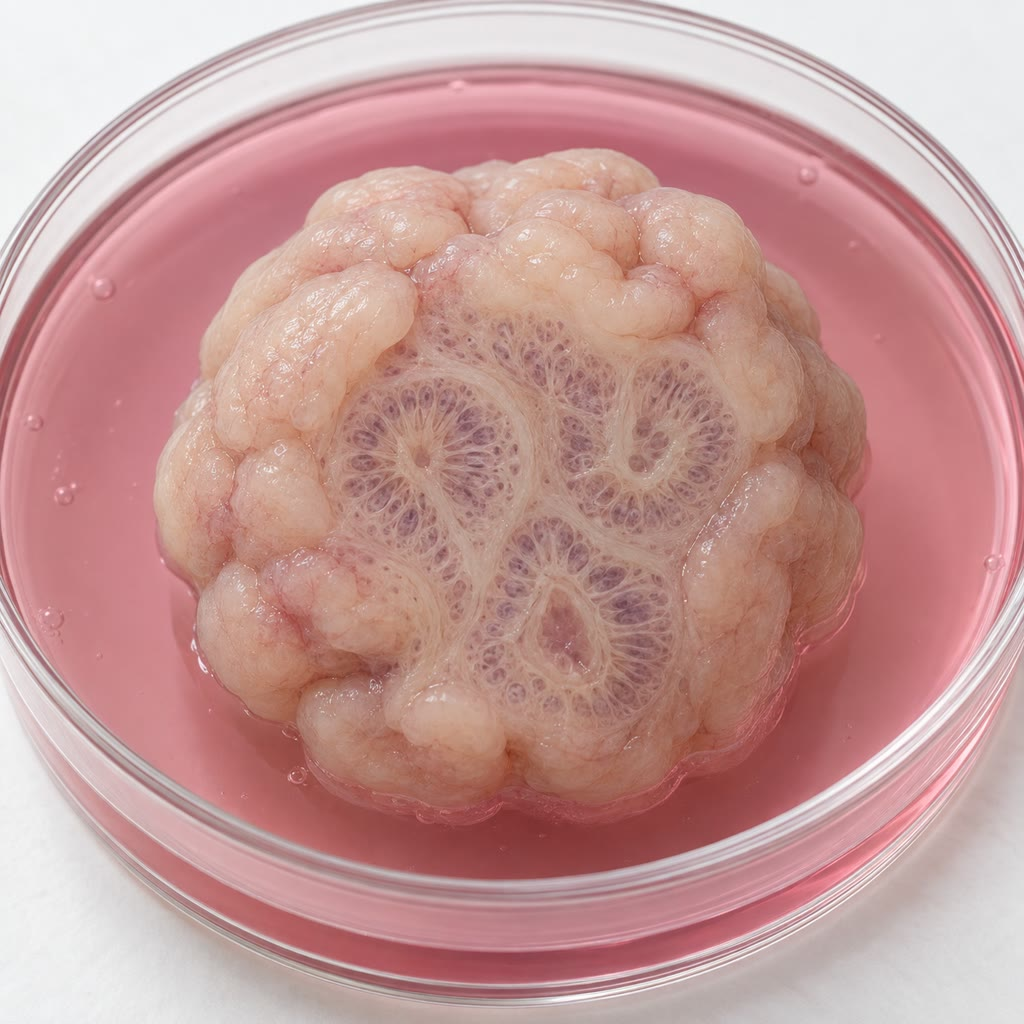
\includegraphics[width=0.4\linewidth]{images/book5/ai/b5-24-brain-organoid.jpg}\hspace{0.04\linewidth}
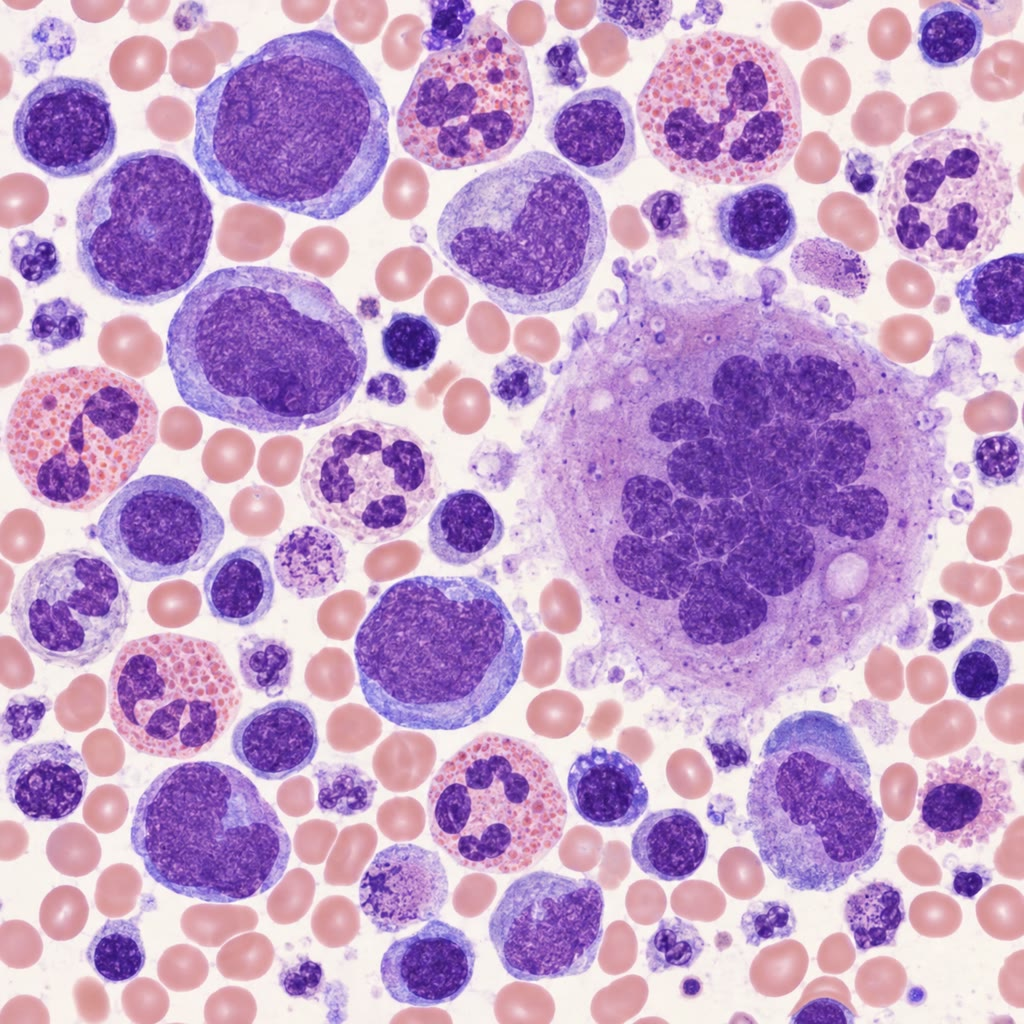
\includegraphics[width=0.4\linewidth]{images/book5/ai/b5-24-bone-marrow-smear.jpg}

{\small À gauche~: un \omterm{def:b3:stem-cells:pluripotency}{organoïde} cérébral cultivé à partir de cellules
pluripotentes humaines --- quelques millimètres de tissu auto-organisé
semblable au cortex, avec des cavités analogues à des ventricules et des
neurones en couches. À droite~: un frottis de moelle osseuse, la
hiérarchie de la première figure vue d'un coup~: blastes, granulocytes
en maturation, précurseurs des globules rouges et un mégacaryocyte.}
\end{omfigure}

\begin{method}[Le traçage de lignée]\label{met:b3:stem-cells:tracing}
\index{traçage de lignée}\index{recombinase Cre}
Pour trouver quelles cellules sont les \omterm{def:b3:stem-cells:stem}{cellules souches} d'un tissu~: (1)
choisir un gène exprimé par les cellules candidates et placer sous son
promoteur une recombinase inductible (Cre-ER, active seulement en
présence de tamoxifène)~; (2) chez le même animal, un gène rapporteur
qui devient définitivement actif quand la recombinase en excise une
cassette d'arrêt --- une couleur héritée par toute la descendance~; (3)
donner une seule dose de tamoxifène pour marquer les cellules candidates
à un instant~; (4) prélever le tissu à intervalles et noter les clones
marqués~: un clone qui grandit, persiste des mois et contient tous les
types cellulaires du tissu vient d'une \omterm{def:b3:stem-cells:stem}{cellule souche}~; un clone largué
en une semaine vient d'une cellule de transit. (5) Avec un rapporteur
multicolore, suivre la compétition entre clones. (6) Éprouver la
fonction directement en tuant les cellules marquées grâce à un récepteur
de toxine exprimé sous le même promoteur, et voir si le tissu cesse de
se renouveler.
\end{method}

\section{La régénération}

\begin{definition}[Comment les animaux repoussent]\label{def:b3:stem-cells:regeneration}
\index{régénération}\index{néoblaste}\index{blastème}\index{dédifférenciation}\index{croissance compensatrice}
La régénération emprunte trois routes. L'\emph{hydre} et la planaire
s'appuient sur des \omterm{def:b3:stem-cells:stem}{cellules souches} adultes pluripotentes~: les
\emph{néoblastes} d'une planaire, un cinquième de ses cellules, sont les
seules cellules en division qu'elle possède, migrent vers une blessure
et rebâtissent n'importe quelle partie manquante, guidés par des signaux
de position (un gradient de Wnt dit au morceau quel bout est la queue~;
bloquez-le et un morceau de queue fait pousser une seconde tête). Les
salamandres rebâtissent un membre à partir d'un \emph{blastème},
calotte de cellules en division au moignon, formée surtout par
\emph{dédifférenciation}~: les fibres musculaires se fragmentent en
cellules mononucléées, les cellules cartilagineuses et conjonctives
reviennent à un état de \omterm{def:b3:stem-cells:stem}{progéniteur}, chacune se souvenant de son tissu
d'origine et de sa position le long du membre, et le blastème
réexécute le programme embryonnaire du membre sous l'épiderme de la
plaie et sous les nerfs, dont la présence est exigée (dénervez le
moignon et rien ne pousse). Le poisson-zèbre refait nageoires et cœur de
la même façon, les cellules musculaires cardiaques survivantes se
divisant pour remplacer un cinquième du ventricule en un mois. Les
mammifères font peu de tout cela~: le foie retrouve sa masse après
l'ablation des deux tiers, mais par la division sur place des cellules
restantes (la \emph{croissance compensatrice}), non en rebâtissant les
lobes perdus~; un bout de doigt régénère chez l'enfant~; les bois du
cerf repoussent chaque année à partir d'un périoste à \omterm{def:b3:stem-cells:stem}{cellules souches}.
Pourquoi pas davantage est une question de compromis~: la réponse
mammifère à une plaie --- coagulation rapide, \omterm{def:b3:innate-immunity:inflammation}{inflammation}, cicatrice
fibroblastique --- ferme vite la plaie contre l'infection et la perte de
sang, et la cicatrice interdit le blastème~; et des cellules qui peuvent
se dédifférencier et se diviser à volonté sont des cellules qui peuvent
devenir des \omterm{def:b3:cancer-biology:hallmarks}{cancers}, un risque qu'un animal à sang chaud et à longue vie
ne peut peut-être pas se payer.
\end{definition}

\begin{omfigure}
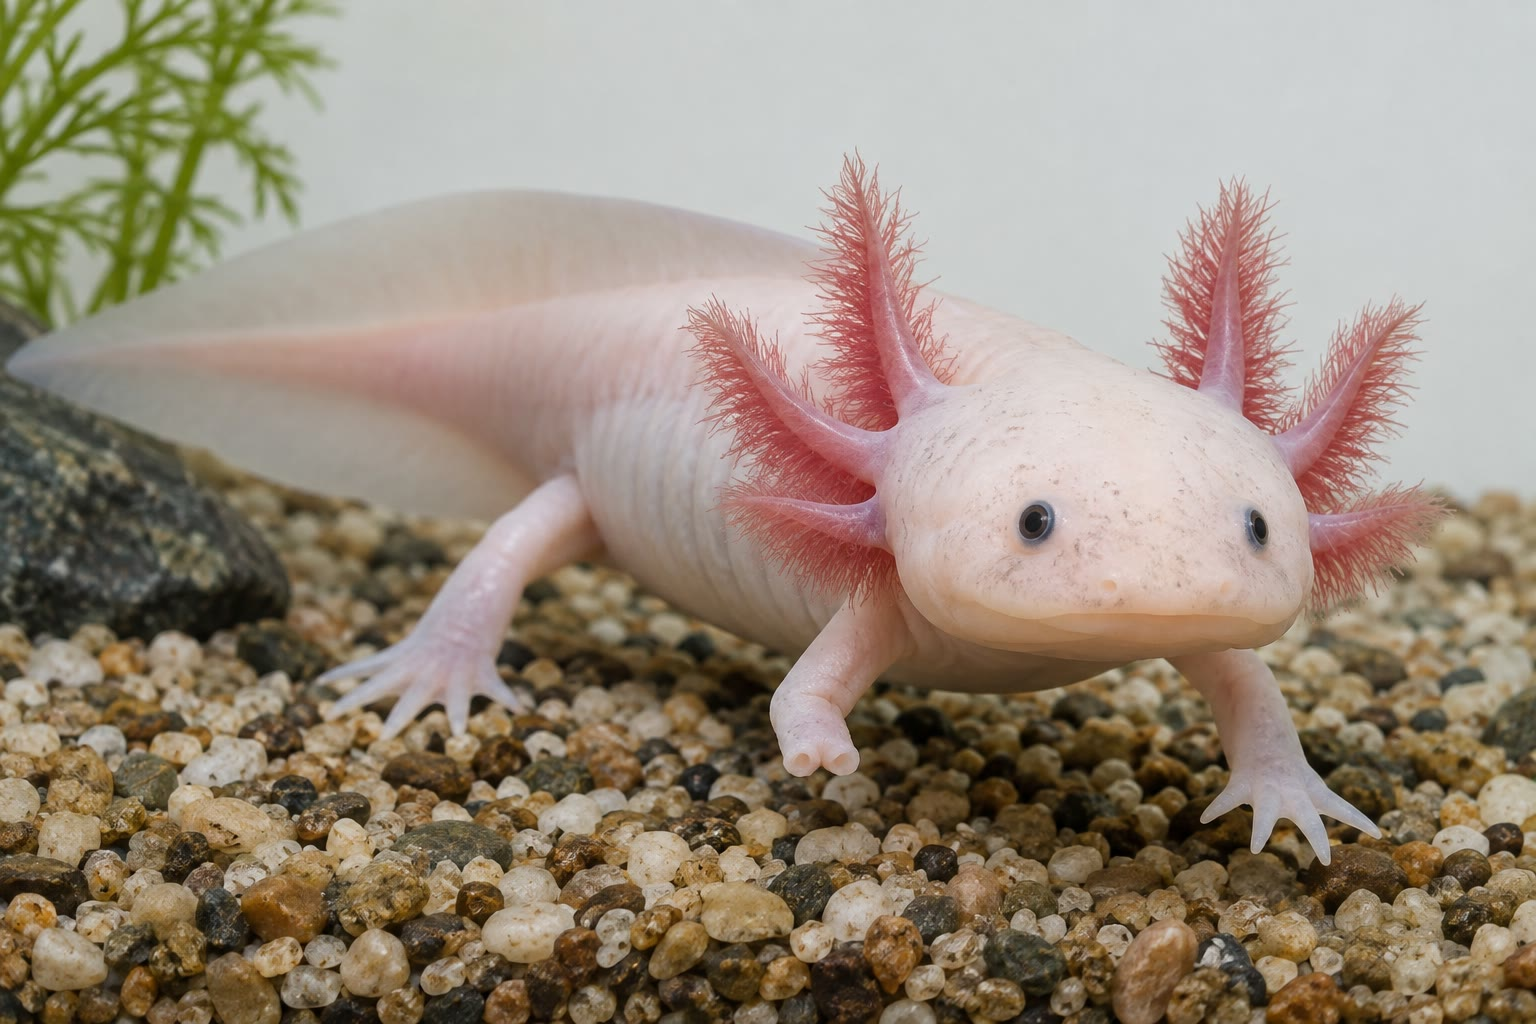
\includegraphics[width=0.46\linewidth]{images/book5/ai/b5-24-axolotl.jpg}\hspace{0.04\linewidth}
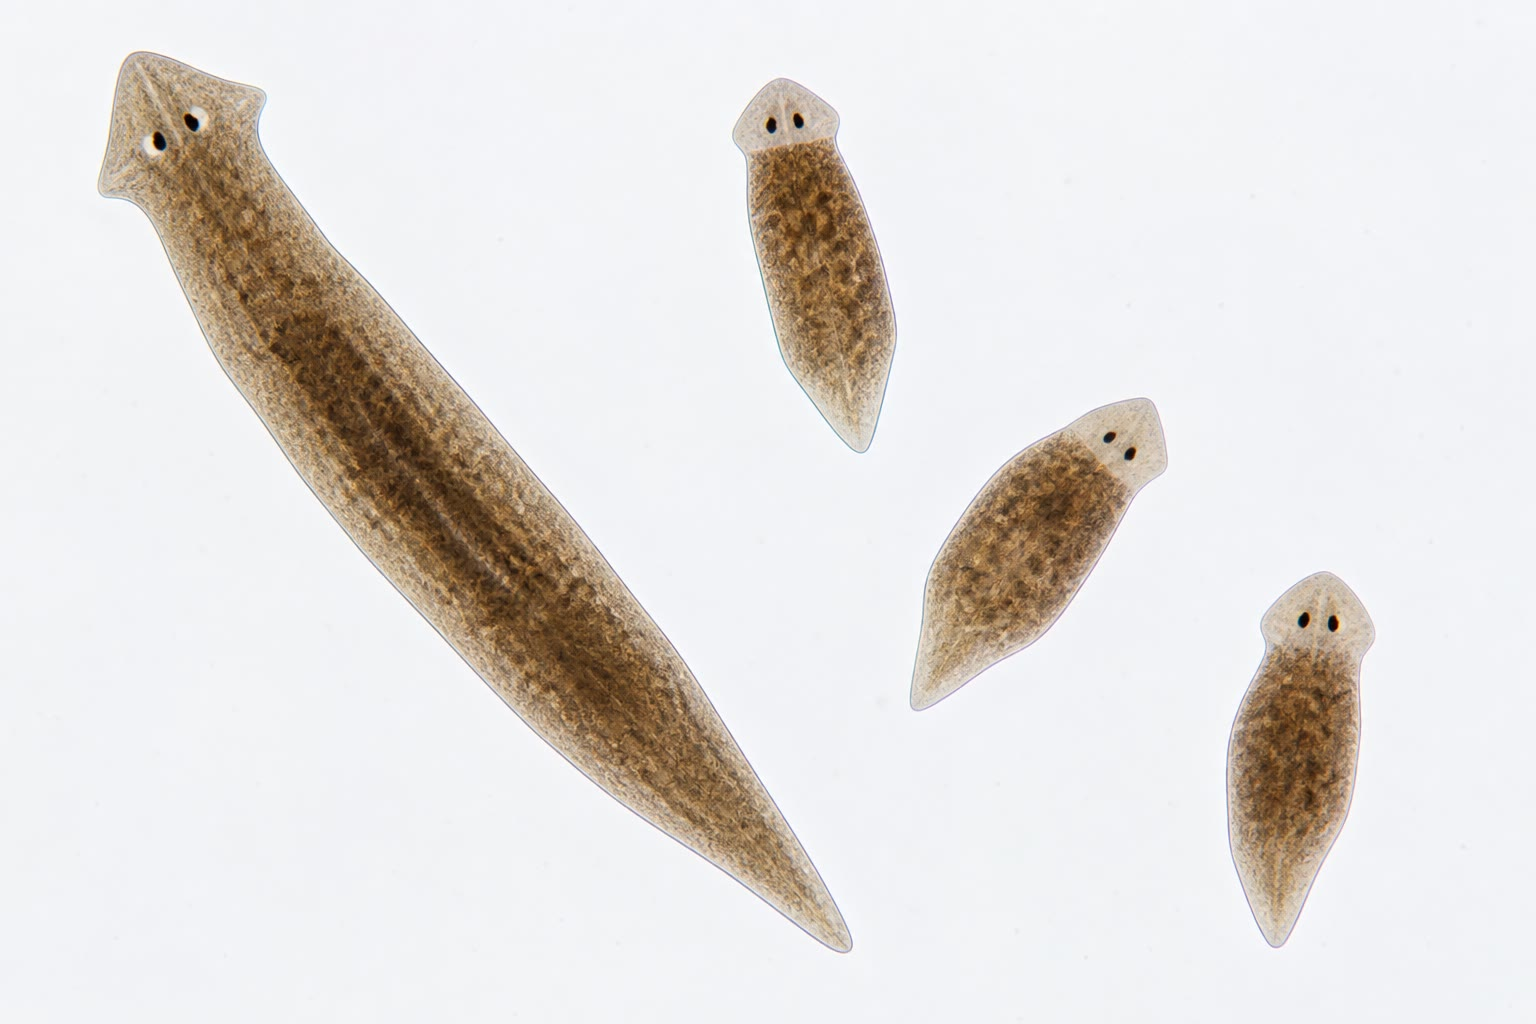
\includegraphics[width=0.46\linewidth]{images/book5/ai/b5-24-planarian-regeneration.jpg}

{\small À gauche~: un axolotl, qui refait pousser un membre en deux mois
à partir d'un \omterm{def:b3:stem-cells:regeneration}{blastème} de cellules dédifférenciées et sait le faire
toute sa vie. À droite~: une planaire coupée en morceaux, chaque morceau
refaisant un ver complet à partir de ses \omterm{def:b3:stem-cells:regeneration}{néoblastes} en deux semaines.}
\end{omfigure}

\begin{proof}[Faits expérimentaux]
Morgan (1898) coupa des planaires en 279 morceaux et trouva que chacun
refaisait un ver entier jusqu'à une limite d'environ un centième du
corps~; Reddien et ses collègues (2011) greffèrent un seul \omterm{def:b3:stem-cells:regeneration}{néoblaste}
dans un ver irradié à dose létale et le rétablirent entièrement --- une
cellule, tous les tissus. Kragl et ses collègues (2009) firent des
axolotls dont les tissus étaient marqués en vert un à un et les
greffèrent sur des hôtes non marqués~: après amputation, le muscle vert
ne donnait que du muscle, le cartilage vert que du cartilage --- le
\omterm{def:b3:stem-cells:regeneration}{blastème} n'est pas un réservoir de cellules pluripotentes mais un
assemblage de \omterm{def:b3:stem-cells:stem}{progéniteurs} restreints à leur lignée, chacun
dédifférencié seulement jusqu'au \omterm{def:b3:stem-cells:stem}{progéniteur} de son propre tissu. Singer
(1952) montra qu'un membre de salamandre ne régénère que si un nombre
seuil de fibres nerveuses atteint le moignon, et que dévier un nerf vers
une plaie du flanc y faisait pousser un membre.
\end{proof}

\section{L'arithmétique du vieillissement}

\begin{theorem}[Les télomères et la limite de Hayflick]\label{thm:b3:stem-cells:hayflick}
\index{télomère}\index{limite de Hayflick}\index{problème de réplication des extrémités}\index{télomérase}\index{sénescence réplicative}
Chaque chromosome se termine par un \emph{télomère}, plusieurs
kilobases de la répétition TTAGGG. Parce que l'ADN polymérase ne peut
achever le dernier tronçon du brin retardé (le \emph{\omterm{thm:b3:stem-cells:hayflick}{problème de
réplication des extrémités}}), chaque division raccourcit chaque télomère
de $\Delta \approx$ \qtyrange{50}{100}{bp}. En partant de
$L_{0} \approx \qty{10}{kb}$ et en déclenchant la \emph{\omterm{thm:b3:stem-cells:hayflick}{sénescence
réplicative}} --- un arrêt définitif imposé par p53 --- quand le télomère
le plus court atteint $L_{\text{crit}} \approx \qty{4}{kb}$, une lignée
cellulaire peut se diviser au plus
\[
n_{\max} = \frac{L_{0} - L_{\text{crit}}}{\Delta} \approx \frac{6000}{50\text{--}100} \approx 60\text{--}120
\]
fois~: la \emph{\omterm{thm:b3:stem-cells:hayflick}{limite de Hayflick}}, la cinquantaine de doublements de
population que les fibroblastes humains accomplissent en culture avant
de s'arrêter. L'enzyme \emph{\omterm{def:b3:cancer-biology:telomerase}{télomérase}}, une transcriptase inverse à
matrice ARN, rallonge les extrémités~; elle est active dans la lignée
germinale, dans les \omterm{def:b3:stem-cells:pluripotency}{cellules souches embryonnaires} et dans bien des
\omterm{def:b3:stem-cells:stem}{cellules souches} adultes, ainsi que dans \qty{90}{\%} des \omterm{def:b3:cancer-biology:hallmarks}{cancers}, qui
ont échappé à la limite en la rallumant. Une \omterm{def:b3:stem-cells:stem}{cellule souche} qui se
divise $d$ fois par an, la \omterm{def:b3:cancer-biology:telomerase}{télomérase} compensant une fraction $f$ de la
perte, dispose de $n_{\max} = (L_{0} - L_{\text{crit}})/[(1 - f)\Delta]$
divisions, et d'une durée de vie de $n_{\max}/d$ ans~: avec $f = 0.7$,
$\Delta
= 60$, $d = 1$, quelque 330 ans pour une \omterm{def:b3:stem-cells:stem}{cellule souche}
hématopoïétique --- mais ses \omterm{def:b3:stem-cells:stem}{progéniteurs}, \omterm{def:b3:cancer-biology:telomerase}{télomérase} éteinte et vingt
divisions jusqu'au globule rouge, dépensent un cinquième de leur réserve
à chaque lignée, et c'est pourquoi les cellules sanguines des personnes
âgées ont des télomères plus courts que celles des jeunes, d'environ
\qty{30}{bp} par an.
\end{theorem}
\begin{proof}
La perte par division est une longueur fixe, de sorte que la longueur du
télomère baisse linéairement avec le numéro de division,
$L_{n} = L_{0} - n\Delta$, et atteint $L_{\text{crit}}$ en
$n = (L_{0} - L_{\text{crit}})/\Delta$~; avec une compensation partielle
la perte nette par division vaut $(1 - f)\Delta$. Hayflick et Moorhead
(1961) ont montré que des fibroblastes humains normaux s'arrêtent après
une cinquantaine de doublements quelles que soient les conditions de
culture, que des cellules congelées après vingt doublements et
décongelées n'accomplissent que les trente restants --- elles comptent
des divisions, non du temps --- et que la limite est plus basse pour des
cellules de donneurs âgés. Harley, Futcher et Greider (1990) ont mesuré
le raccourcissement des télomères avec les doublements en culture et
avec l'âge du donneur~; Bodnar et ses collègues (1998) ont mis de la
\omterm{def:b3:cancer-biology:telomerase}{télomérase} dans des cellules normales, qui se sont divisées indéfiniment
au-delà de la limite sans devenir cancéreuses, ce qui a établi le
télomère comme l'horloge.
\end{proof}

\begin{omfigure}
\begin{tikzpicture}
\begin{axis}[
  width=0.62\linewidth, height=5.4cm,
  axis x line=bottom, axis y line=left,
  xmin=0, xmax=120, ymin=0, ymax=11,
  xlabel={doublements de population}, ylabel={longueur des télomères (kb)},
  xlabel style={font=\small, at={(axis description cs:0.5,-0.12)}, anchor=north}, ylabel style={font=\small},
  tick label style={font=\small}, xtick={0,30,60,90,120}, ytick={4,7,10},
  clip=false,
]
\addplot[very thick, omDef, domain=0:60, samples=2] {10-0.1*x};
\addplot[very thick, omThm, domain=0:120, samples=2] {10-0.05*x};
\addplot[very thick, omMeth!70!black, domain=0:120, samples=2] {10-0.015*x};
\draw[dashed, gray] (axis cs:0,4) -- (axis cs:120,4); \node[font=\scriptsize, gray, anchor=north west] at (axis cs:2,3.9) {sénescence à $L_{\text{crit}} = \qty{4}{kb}$};
\node[font=\scriptsize, omDef, anchor=south west] at (axis cs:63,4.3) {$\Delta = \qty{100}{bp}$~: 60 doublements};
\node[font=\scriptsize, omThm, anchor=west] at (axis cs:70,8.0) {$\Delta = \qty{50}{bp}$~: 120};
\node[font=\scriptsize, omMeth!70!black, anchor=south west, align=left] at (axis cs:78,9.3) {télomérase compensant\\\qty{70}{\%}~: 400};
\fill[omDef] (axis cs:60,4) circle (2pt); \fill[omThm] (axis cs:120,4) circle (2pt);
\end{axis}
\end{tikzpicture}

{\small Les télomères comme compteur de divisions. Une perte fixe par
division donne une droite~; là où elle croise la longueur critique la
lignée s'arrête. La \omterm{def:b3:cancer-biology:telomerase}{télomérase} aplatit la pente et, pleinement active,
abolit la limite --- dans la lignée germinale, et dans les \omterm{def:b3:cancer-biology:hallmarks}{cancers}.}
\end{omfigure}

\begin{proposition}[La loi de Gompertz]\label{prop:b3:stem-cells:gompertz}
\index{loi de Gompertz}\index{taux de mortalité}\index{marqueurs du vieillissement}\index{cellule sénescente}
Au-delà d'une trentaine d'années le taux de mortalité humain $\mu(t)$
--- la probabilité de mourir dans l'année qui vient --- double tous les
huit ans~: $\mu(t) =
\mu_{0}\,\mathrm{e}^{\gamma(t - t_{0})}$ avec $\gamma = \ln 2/8 \approx
\qty{0.087}{yr^{-1}}$ (Gompertz, 1825). La survie jusqu'à l'âge $t$ vaut
alors
\[
S(t) = \exp\!\Bigl[-\frac{\mu_{0}}{\gamma}\bigl(\mathrm{e}^{\gamma(t - t_{0})} - 1\bigr)\Bigr],
\]
courbe plate pendant des décennies puis chutant brutalement, avec une
espérance de vie médiane
$t_{1/2} = t_{0} + \gamma^{-1}\ln(1 + \gamma\ln 2/\mu_{0})$~: pour
$\mu_{0} = 10^{-3}$ par an à trente ans, environ $30 + 47 = 77$ ans. La
même loi, avec d'autres constantes, vaut pour la souris (doublement en
trois mois), le chien, la mouche et le ver~: le vieillissement est une
montée exponentielle de la vulnérabilité, non une horloge qui s'arrête.
La biologie derrière l'exposant est un jeu de \emph{marqueurs} qui
interagissent~: dégâts de l'ADN accumulés et dérive \omterm{def:b3:chromatin-epigenetics:epigenetics}{épigénétique},
attrition des télomères, perte de la protéostasie, déclin
mitochondrial, épuisement des réservoirs de \omterm{def:b3:stem-cells:stem}{cellules souches},
accumulation de \emph{\omterm{prop:b3:stem-cells:gompertz}{cellules sénescentes}} qui ne se divisent plus mais
sécrètent des signaux inflammatoires, et \omterm{def:b3:innate-immunity:inflammation}{inflammation} chronique~; chez
la souris, éliminer les \omterm{prop:b3:stem-cells:gompertz}{cellules sénescentes} ou restreindre les calories
allonge la vie, et chez le ver une seule mutation de la voie de type
\omterm{def:b3:endocrinology:glucose}{insuline} la double. Savoir si l'exposant peut être abaissé chez l'humain,
plutôt que la constante $\mu_{0}$ que la médecine a divisée par dix en un
siècle, est la question ouverte.
\end{proposition}
\begin{proof}
Si $\mu$ désigne le risque instantané, alors
$\mathrm{d}S/\mathrm{d}t = -\mu(t)S$ et $\ln S =
-\int_{t_{0}}^{t}\mu = -(\mu_{0}/\gamma)(\mathrm{e}^{\gamma(t-t_{0})} -
1)$. En posant $S = 1/2$~: $\mathrm{e}^{\gamma(t-t_{0})} = 1 + \gamma\ln 2/
\mu_{0}$, d'où la médiane~; avec $\gamma = 0.087$ et $\mu_{0} =
10^{-3}$, $\ln(1 + 60) = 4.1$, $t - t_{0} = 47$. La loi empirique est
l'ajustement de Gompertz aux tables de mortalité anglaises~; qu'elle
décrive tant d'espèces avec une forme commune et des constantes propres
à chacune est admis ici comme le résumé d'un siècle de démographie.
\end{proof}

\begin{omfigure}
\begin{tikzpicture}
\begin{semilogyaxis}[
  width=0.5\linewidth, height=5.2cm,
  axis x line=bottom, axis y line=left,
  xmin=20, xmax=100, ymin=0.0003, ymax=1,
  xlabel={âge (années)}, ylabel={taux de mortalité par an},
  xlabel style={font=\small, at={(axis description cs:0.5,-0.12)}, anchor=north}, ylabel style={font=\small},
  tick label style={font=\small}, xtick={30,50,70,90}, ytick={0.001,0.01,0.1,1}, yticklabels={0.001,0.01,0.1,1},
  clip=false,
]
\addplot[very thick, omDef, domain=30:100, samples=2] {0.001*exp(0.0866*(x-30))};
\node[font=\scriptsize, omDef, anchor=north west, align=left] at (axis cs:32,0.3) {$\mu = \mu_{0}\,\mathrm{e}^{\gamma(t-30)}$\\doublement tous les 8 ans};
\end{semilogyaxis}
\begin{axis}[
  at={(0.55\linewidth,0)}, anchor=south west,
  width=0.43\linewidth, height=5.2cm,
  axis x line=bottom, axis y line=left,
  xmin=20, xmax=110, ymin=0, ymax=1.05,
  xlabel={âge (années)}, ylabel={fraction de survivants},
  xlabel style={font=\small, at={(axis description cs:0.5,-0.12)}, anchor=north}, ylabel style={font=\small},
  tick label style={font=\small}, xtick={30,50,77,100}, ytick={0.5,1},
  clip=false,
]
\addplot[very thick, omThm, domain=30:110, samples=80] {exp(-(0.001/0.0866)*(exp(0.0866*(x-30))-1))};
\draw[dashed, gray] (axis cs:77,0) -- (axis cs:77,0.5) -- (axis cs:20,0.5);
\node[font=\scriptsize, omThm, anchor=north east, align=right] at (axis cs:75,0.45) {médiane\\77 ans};
\end{axis}
\end{tikzpicture}

{\small La \omterm{prop:b3:stem-cells:gompertz}{loi de Gompertz}. À gauche~: sur un axe logarithmique le taux
de mortalité est une droite à partir de trente ans. À droite~: la courbe
de survie qui s'ensuit --- un plateau, puis une falaise, avec la médiane
là où l'intégrale du risque atteint $\ln 2$.}
\end{omfigure}

\begin{remark}[Le renouvellement et son prix]\label{rem:b3:stem-cells:remark}
Un corps qui se renouvelle doit garder des cellules capables de se
diviser indéfiniment, et des cellules capables de se diviser
indéfiniment sont la matière du \omterm{def:b3:cancer-biology:hallmarks}{cancer}~; un corps qui se garde du \omterm{def:b3:cancer-biology:hallmarks}{cancer}
en comptant les divisions et en imposant la \omterm{def:b3:cell-cycle-apoptosis:other}{sénescence} doit, avec le
temps, manquer de cellules capables de se diviser. La hiérarchie des
\omterm{def:b3:stem-cells:stem}{cellules souches} est une solution --- peu de cellules lentes protégées
dans des \omterm{def:b3:stem-cells:stem}{niches}, beaucoup de cellules rapides qui meurent vite --- et la
\omterm{thm:b3:stem-cells:hayflick}{limite de Hayflick} une autre, et l'exponentielle de Gompertz est la
somme de leurs coûts. La salamandre paie autrement~: elle tolère des
cellules qui se dédifférencient et refait pousser une patte, et elle est
à sang froid, lente et vit rarement assez longtemps pour payer la note
du \omterm{def:b3:cancer-biology:hallmarks}{cancer}. Les cellules avec lesquelles vous êtes né ne sont, pour
l'essentiel, pas celles que vous avez~; celles qui ont fait les
remplaçantes sont celles qu'il vous faut garder.
\end{remark}

\section{Exercices}

\begin{exercise}[$\star$]\label{exo:b3:stem-cells:1}
Définir l'\omterm{def:b3:stem-cells:stem}{auto-renouvellement}, la potence, la \omterm{def:b3:stem-cells:stem}{niche} et la \omterm{def:b3:stem-cells:stem}{cellule
d'amplification transitoire}, et donner un exemple de chacun dans
l'intestin.
\end{exercise}

\begin{exercise}[$\star$]\label{exo:b3:stem-cells:2}
Qu'a montré le test des colonies spléniques, et quelle propriété d'une
\omterm{def:b3:stem-cells:stem}{cellule souche} a exigé une seconde souris pour être démontrée~?
\end{exercise}

\begin{exercise}[$\star$]\label{exo:b3:stem-cells:3}
Nommer les quatre facteurs de Yamanaka et expliquer pourquoi la
\omterm{def:b3:stem-cells:pluripotency}{reprogrammation} prend des semaines et réussit dans une cellule sur mille.
\end{exercise}

\begin{exercise}[$\star$]\label{exo:b3:stem-cells:4}
Opposer les routes de la planaire et de la salamandre vers la
\omterm{def:b3:stem-cells:regeneration}{régénération}, et dire ce que les greffes de Kragl ont montré du \omterm{def:b3:stem-cells:regeneration}{blastème}.
\end{exercise}

\begin{exercise}[$\star\star$]\label{exo:b3:stem-cells:5}
Les télomères partent de \qty{11}{kb}, la \omterm{def:b3:cell-cycle-apoptosis:other}{sénescence} survient à
\qty{5}{kb}, la perte vaut \qty{75}{bp} par division. \omterm{thm:b3:stem-cells:hayflick}{Limite de
Hayflick}~? Des cellules d'un donneur de 70 ans ont \qty{8}{kb}~:
doublements restants~? Si la \omterm{def:b3:cancer-biology:telomerase}{télomérase} compense \qty{60}{\%} de la
perte, quelle limite~?
\end{exercise}

\begin{exercise}[$\star\star$]\label{exo:b3:stem-cells:6}
Une crypte contient 14 \omterm{def:b3:stem-cells:stem}{cellules souches} qui se divisent une fois par
jour, alimentant des cellules de transit qui se divisent 4 fois de plus,
et la crypte fournit \num{300} cellules par jour à sa villosité.
Vérifier l'arithmétique~: combien de divisions de \omterm{def:b3:stem-cells:stem}{cellules souches} par
jour produisent des filles en différenciation, et cela fait combien de
\omterm{def:b3:stem-cells:stem}{cellules souches} en équivalent de divisions~?
\end{exercise}

\begin{exercise}[$\star\star$]\label{exo:b3:stem-cells:7}
Le corps fabrique $2\times 10^{11}$ globules rouges par jour, chacun au
bout d'une vingtaine de divisions depuis une \omterm{def:b3:stem-cells:stem}{cellule souche}. Combien de
divisions de \omterm{def:b3:stem-cells:stem}{cellules souches} par jour cela exige-t-il et, avec
\num{10000} \omterm{def:b3:stem-cells:stem}{cellules souches}, à quelle fréquence chacune se divise-t-elle~?
Comparer à l'«~environ une fois par an~» observé et expliquer l'écart.
\end{exercise}

\begin{exercise}[$\star\star$]\label{exo:b3:stem-cells:8}
Avec $\gamma = \qty{0.087}{yr^{-1}}$ et $\mu_{0} = 10^{-3}$ à trente
ans, calculer le taux de mortalité à 50, 70 et 90 ans, la survie à 70 et
90 ans, et l'espérance de vie médiane. Que fait la division par deux de
$\mu_{0}$ à la médiane~? Et celle de $\gamma$~?
\end{exercise}

\begin{exercise}[$\star\star$]\label{exo:b3:stem-cells:9}
On retire les deux tiers du foie d'un rat. Les hépatocytes restants, qui
se divisent tous, en rétablissent la masse en dix jours. Combien de
divisions faut-il à chacun~? Pourquoi appelle-t-on cela une \omterm{def:b3:stem-cells:regeneration}{croissance
compensatrice} et non une \omterm{def:b3:stem-cells:regeneration}{régénération}, et que le foie ne rebâtit-il
\emph{pas}~?
\end{exercise}

\begin{exercise}[$\star\star\star$]\label{exo:b3:stem-cells:10}
\omterm{prop:b3:stem-cells:crypt}{Dérive neutre}~: $N$ \omterm{def:b3:stem-cells:stem}{cellules souches} d'une \omterm{def:b3:stem-cells:stem}{niche} se divisent
symétriquement~; à chaque événement une cellule se divise et une est
perdue au hasard, de sorte que l'effectif d'un clone donné suit une
marche au hasard entre $0$ et $N$. Argumenter que la probabilité qu'un
clone de $k$ cellules finisse par prendre toute la \omterm{def:b3:stem-cells:stem}{niche} vaut $k/N$, et
qu'avec $N = 14$ un clone d'une seule cellule a une probabilité $1/14$. Que
cela prédit-il du sort d'une \omterm{def:b3:stem-cells:stem}{cellule souche} porteuse d'une nouvelle
mutation neutre~?
\end{exercise}

\begin{exercise}[$\star\star\star$]\label{exo:b3:stem-cells:11}
Une mutation donne à un clone de \omterm{def:b3:stem-cells:stem}{cellules souches} un avantage de
\qty{10}{\%} dans la compétition de l'\cref{exo:b3:stem-cells:10}.
Expliquer qualitativement pourquoi sa probabilité de prise de contrôle
monte bien au-dessus de $k/N$, pourquoi les cryptes et la moelle des
personnes âgées sont de plus en plus dominées par quelques clones
(l'hématopoïèse clonale), et pourquoi c'est un premier pas vers le
\omterm{def:b3:cancer-biology:hallmarks}{cancer} sans être un \omterm{def:b3:cancer-biology:hallmarks}{cancer}.
\end{exercise}

\begin{exercise}[$\star\star\star$]\label{exo:b3:stem-cells:12}
Supposons que l'exposant de Gompertz $\gamma$ reflète une vitesse
d'accumulation des dégâts et la constante $\mu_{0}$ l'environnement. La
médecine a divisé $\mu_{0}$ par dix depuis 1900 sans changer $\gamma$.
Calculer le gain d'espérance de vie médiane que donne cette division par
dix, et le gain supplémentaire d'une nouvelle division par dix~;
expliquer pourquoi les rendements décroissent, et ce que ferait à la
place une baisse de \qty{20}{\%} de $\gamma$.
\end{exercise}

\section{Problème~: les cellules avec lesquelles vous êtes né}

\begin{problem}[{Problème du week-end --- le renouvellement d'un corps en
chiffres~: la hiérarchie du sang et ce qu'elle demande à ses cellules
souches, la dérive de la crypte, l'horloge télomérique et la façon dont
la télomérase et les progéniteurs la dépensent, la courbe de Gompertz de
la population, et les compromis qu'accepte un animal qui régénère, pour
finir sur le compte de Hayflick, la réserve d'une vie de cellule souche
et l'espérance de vie médiane}]
\label{pb:b3:stem-cells:1}
Données~: globules rouges $2.5\times 10^{11}$ par jour, granulocytes
$10^{11}$ par jour~; $20$ divisions de la \omterm{def:b3:stem-cells:stem}{cellule souche} à la cellule
mûre~; \num{10000} \omterm{def:b3:stem-cells:stem}{cellules souches} hématopoïétiques. Télomères~:
$L_{0} = \qty{10}{kb}$, $L_{\text{crit}} = \qty{4}{kb}$,
$\Delta = \qty{60}{bp}$ par division~; la \omterm{def:b3:cancer-biology:telomerase}{télomérase} des \omterm{def:b3:stem-cells:stem}{cellules souches}
compense $f = 0.7$~; aucune dans les \omterm{def:b3:stem-cells:stem}{progéniteurs}. Crypte~: $N = 14$
\omterm{def:b3:stem-cells:stem}{cellules souches}, une division par jour. Gompertz~: $\mu_{0} =
10^{-3}$ par an à 30 ans, $\gamma = \qty{0.087}{yr^{-1}}$. Membre
d'axolotl~: \qty{40}{mm} repoussés en \qty{60}{d}~; \omterm{def:b3:stem-cells:regeneration}{blastème} de
$10^{5}$ cellules passant à $10^{8}$.

\medskip
\noindent\textbf{Partie I --- Le sang.}
\begin{enumerate}
  \item Cellules produites par jour au total, et par seconde.
  \item Chaque cellule mûre est le terme de $20$ divisions~: combien de
        cellules résultent d'une fille engagée d'une \omterm{def:b3:stem-cells:stem}{cellule souche}~?
        Combien de filles engagées faut-il par jour~?
  \item Avec \num{10000} \omterm{def:b3:stem-cells:stem}{cellules souches}, combien de divisions
        différenciantes par \omterm{def:b3:stem-cells:stem}{cellule souche} et par jour cela implique-t-il~?
        Et par an~?
  \item La division des \omterm{def:b3:stem-cells:stem}{cellules souches} mesurée est d'environ une fois
        par an. Concilier~: que doivent faire les \omterm{def:b3:stem-cells:stem}{progéniteurs} que le
        calcul de la question~3 supposait fait par les \omterm{def:b3:stem-cells:stem}{cellules souches}~?
  \item Les \omterm{def:b3:stem-cells:stem}{progéniteurs} n'ont pas de \omterm{def:b3:cancer-biology:telomerase}{télomérase}. En partant de
        \qty{10}{kb}, quelle longueur de télomère un précurseur de
        globule rouge atteint-il après ses $20$ divisions~? Importe-t-il
        qu'elle soit au-dessus de $L_{\text{crit}}$~?
  \item Une \omterm{def:b3:stem-cells:stem}{cellule souche} qui se divise une fois par an avec $f = 0.7$~:
        perte nette par division, divisions jusqu'à la \omterm{def:b3:cell-cycle-apoptosis:other}{sénescence}, et
        années. Commenter.
\end{enumerate}

\medskip
\noindent\textbf{Partie II --- La crypte.}
\begin{enumerate}[resume]
  \item Divisions par crypte et par jour à l'étage des \omterm{def:b3:stem-cells:stem}{cellules
        souches}~; si la moitié des événements remplacent une \omterm{def:b3:stem-cells:stem}{cellule
        souche} perdue et l'autre moitié alimentent la zone de transit,
        combien de cellules engagées par jour, et combien de cellules de
        villosité après $4$ divisions de transit~?
  \item La probabilité de prise de contrôle d'un clone d'une seule
        cellule vaut $1/N$. Le temps attendu jusqu'à la monoclonalité est
        de l'ordre de $N^{2}$ événements de division par cellule~;
        l'estimer en jours et le comparer aux observations de confetti
        (quelques mois).
  \item Une \omterm{def:b3:stem-cells:stem}{cellule souche} acquiert une mutation. Probabilité qu'elle
        finisse fixée dans sa crypte~? Dans combien des $10^{7}$ cryptes
        d'un côlon une mutation apparue une fois par crypte se
        fixerait-elle~?
  \item Pourquoi la dérive d'une crypte protège-t-elle mieux du \omterm{def:b3:cancer-biology:hallmarks}{cancer}
        qu'un tissu où chaque \omterm{def:b3:stem-cells:stem}{cellule souche} se divise asymétriquement à
        vie~?
  \item Après qu'une irradiation a tué les \omterm{def:b3:stem-cells:stem}{cellules souches}, les
        cellules de transit reviennent en arrière et remplissent la
        \omterm{def:b3:stem-cells:stem}{niche}. Que cela dit-il du lieu où réside le caractère souche~?
  \item Esquisser l'expérience de \omterm{met:b3:stem-cells:tracing}{traçage de lignée} qui distingue la
        dérive symétrique de la \omterm{def:b3:stem-cells:stem}{division asymétrique}, et les deux issues.
\end{enumerate}

\medskip
\noindent\textbf{Partie III --- L'horloge.}
\begin{enumerate}[resume]
  \item \omterm{thm:b3:stem-cells:hayflick}{Limite de Hayflick} d'une lignée somatique sans \omterm{def:b3:cancer-biology:telomerase}{télomérase}.
  \item Une culture de fibroblastes est congelée après $25$ doublements
        et décongelée dix ans plus tard~: doublements restants~? Que
        montre cela de ce que compte la cellule~?
  \item Les télomères des leucocytes raccourcissent de \qty{30}{bp} par
        an chez l'adulte. En partant de \qty{8}{kb} à vingt ans, quand
        atteindraient-ils $L_{\text{crit}}$~? Comparer à la durée de vie
        et commenter.
  \item De la \omterm{def:b3:cancer-biology:telomerase}{télomérase} ajoutée à des fibroblastes normaux leur permet
        de passer la limite sans devenir cancéreux. La \omterm{def:b3:cancer-biology:telomerase}{télomérase} est
        active dans \qty{90}{\%} des \omterm{def:b3:cancer-biology:hallmarks}{cancers}. Concilier les deux énoncés.
  \item Calculer le taux de mortalité de Gompertz à 40, 60, 80 et 100
        ans, et la survie à chacun.
  \item Espérance de vie médiane~; et l'âge auquel \qty{10}{\%}
        survivent.
\end{enumerate}

\medskip
\noindent\textbf{Partie IV --- Refaire pousser.}
\begin{enumerate}[resume]
  \item Axolotl~: vitesse moyenne de repousse en mm/jour~; doublements
        pour que le \omterm{def:b3:stem-cells:regeneration}{blastème} passe de $10^{5}$ à $10^{8}$ cellules, et
        temps de doublement moyen sur 60 jours.
  \item Si les cellules dédifférenciées se divisaient comme celles du
        \omterm{def:b3:stem-cells:regeneration}{blastème} toute la vie et qu'une division porte une chance de
        $10^{-9}$ par cellule d'une mutation \omterm{def:b3:cancer-biology:genes}{oncogène}, combien de telles
        mutations apparaissent en une \omterm{def:b3:stem-cells:regeneration}{régénération}~? Pourquoi l'axolotl
        n'est-il pourtant presque jamais cancéreux, et pourquoi un
        mammifère ne s'en tirerait-il peut-être pas ainsi~?
  \item Dénerver le moignon arrête la \omterm{def:b3:stem-cells:regeneration}{régénération}. Proposer une
        expérience montrant que le nerf fournit un facteur diffusible, et
        une identité possible de ce facteur.
  \item Un morceau de queue de planaire fait pousser une seconde queue au
        lieu d'une tête quand on invalide un inhibiteur de Wnt.
        Expliquer par un gradient et la mémoire de position du morceau.
  \item Foie humain après une résection des deux tiers~: fraction des
        hépatocytes qui doivent se diviser une fois, deux fois, pour
        rétablir la masse. Pourquoi le résultat est-il un foie qui
        fonctionne mais de la mauvaise forme~?
  \item Pourquoi un corps qui régénérerait comme un axolotl aurait-il une
        autre courbe de Gompertz, et dans quel sens~?
  \item Résumer~: le compte de Hayflick (question~13), les divisions et
        les années d'une \omterm{def:b3:stem-cells:stem}{cellule souche} aidée par la \omterm{def:b3:cancer-biology:telomerase}{télomérase}
        (question~6), et l'espérance de vie médiane (question~18).
\end{enumerate}
\end{problem}
